\documentclass[onlytextwidth, aspectratio=169]{beamer}
\usepackage[utf8]{inputenc}
\usepackage{microtype}
\usepackage{amsmath}
\usepackage{amssymb}
\usepackage[nomessages]{fp} %\FPeval{\var-name}{2*sin(pi/6)}
\usepackage{siunitx} %units in math. eg 20\milli\meter
\usepackage{yhmath} % for arcs, overparenth command
\usepackage{tikz} %graphics
\usetikzlibrary{quotes, angles, arrows, arrows.meta}
%\usepackage{graphicx} already loaded by beamer class
%consider setting \graphicspath{{images/}}
%\parskip ?? to avoid paragraph indent
\usepackage{multicol} %may not need this package, just columns environment
\usepackage{venndiagram}

\subtitle[BECA]{Bronx Early College Academy}
\author[Huson]{Christopher J. Huson PhD}

\setbeamertemplate{headline}{\vskip2mm 
  \, BECA / \insertshortauthor \, / \inserttitle
  \hfill 
  \insertsection
  }

%Tick mark commands
\newcommand\ticks{}
  \def\ticks{{Bar[scale=2]}-{Bar[scale=2]}}
\newcommand\paraticks{}
  \def\paraticks{{Straight Barb[reversed, scale=2]}-{Straight Barb[scale=2]}}

\title{Geometry Unit 4: Volume}
\date{31 October - 18 November 2022}

\begin{document}
\frame{\titlepage}
\section[Outline]{}
\frame{\tableofcontents}

\section{4.1 Nets \hfill 31 October \,}
\begin{frame}{Learning Target: I can fold nets into 3-dimensional solids}
  {HSG.CO.C.9 Prove theorems about lines and angles  \hfill \alert{4.1 Monday 31 October}}
  \begin{block}{Do Now}
    \begin{enumerate}
      \item Review your Deltamath assignments
      \item Check your Jumprope scores
      \item Set a study goal
      \item Answer survey in Google Classroom, ``Mark as Done''
    \end{enumerate}
  \end{block}
    Lesson: Nets, Deltamath classwork practice \\
    Homework: Area formulas review problem set
\end{frame}

\section{4.2 Rectangular prisms \hfill 1 November \,}
\begin{frame}{Learning Target: I can calculate the volume of a \emph{rectangular prism}}
  {HSG.CO.C.9 Prove theorems about lines and angles  \hfill \alert{4.2 Tuesday 1 November}}
  \begin{block}{Do Now}
    \begin{enumerate}
      \item Find the area of a rectangle 4 inches by 6 inches
      \item Find the length of a rectangle 7 inches wide with an area of 63 square inches
    \end{enumerate}
  \end{block}
    Lesson: Prism definitions, volume formula \\
    Homework: Deltamath practice
\end{frame}

\begin{frame}{A prism is a polyhedron, a 3-dimensional shape}
    \begin{columns}
      \column{0.7\textwidth}
      \begin{description}
        \item[Solid] A 3-dimensional object
        \item[Face] A flat surface of a geometric solid
        \item[Edge] A line segment where two faces meet
        \item[Vertex] A point where edges meet 
        \item[Prism] A solid with two identical, parallel, bases and uniform cross section
        \item[Base] Flat shapes that form the top and bottom or ends of a prism
        \item[Lateral face] The sides of a prism, which are parallelograms
        \item[Cross section] The shape of a plane's intersection with a solid
      \end{description}
      \column{0.3\textwidth}
      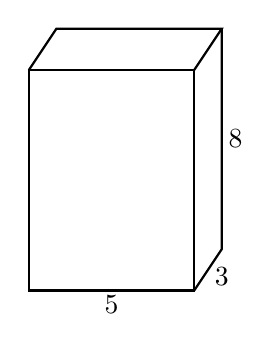
\begin{tikzpicture}[scale=0.7]
        \draw [-, thick] (0,0)--(3,0)--(3,4)--(0,4)--cycle;
        \draw [-, thick] (0,4)--(0.5,4.75)--(3.5,4.75)--(3,4);
        \draw [-, thick] (3,0)--(3.5,0.75)--(3.5,4.75);
        \node at (3.75, 2.75){$8$};
        \node at (1.5, -0.25){$5$};
        \node at (3.5, 0.25){$3$};
      \end{tikzpicture}
    \end{columns} \vspace{0.5cm}
  \end{frame}

\begin{frame}{Common types of prisms, named by their base}
  \begin{columns}
    \column{0.7\textwidth}
    \begin{description}
      \item[Rectangular] Bases are rectangles (or squares)
      \item[Triangular] Triangular base
      \item[Hexagonal] Six-sided base, a hexagon
      \item[Cylinder] Solid with two parallel circles as bases 
      \item[Right] Lateral faces are a right angles to the base
      \item[Oblique] Slanted
    \end{description}
    \column{0.3\textwidth}
    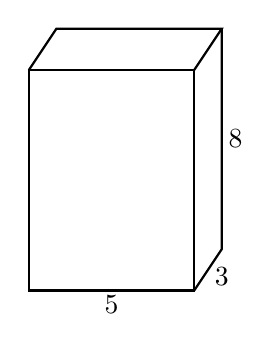
\begin{tikzpicture}[scale=0.7]
      \draw [-, thick] (0,0)--(3,0)--(3,4)--(0,4)--cycle;
      \draw [-, thick] (0,4)--(0.5,4.75)--(3.5,4.75)--(3,4);
      \draw [-, thick] (3,0)--(3.5,0.75)--(3.5,4.75);
      \node at (3.75, 2.75){$8$};
      \node at (1.5, -0.25){$5$};
      \node at (3.5, 0.25){$3$};
    \end{tikzpicture}
  \end{columns} \vspace{0.5cm}
  \href{https://mathmonks.com/prism}{Math Monks prisms page}
\end{frame}

\begin{frame}
  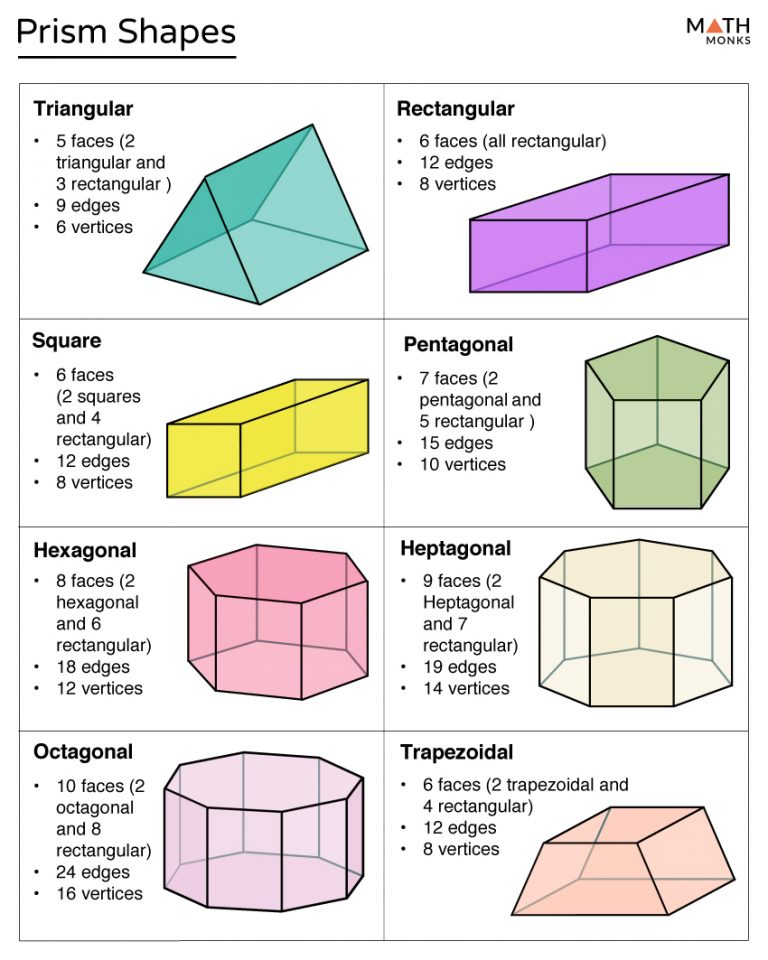
\includegraphics[width=0.5\textwidth]{../graphics/prism-shapes-768x960.jpeg}
\end{frame}

\begin{frame}{Volume is a measure of space, the number of unit cubes a solid contains}
  Given the area of the base $B$ and height $h$, \\
  the volume of a prism is $V= B \times h$
  \vspace{0.5cm}
  \begin{columns}
    \column{0.7\textwidth}
    \begin{description}
      \item[Rectangular] $V= l \times w \times h$
      \item[Square] $V= s^2 \times h$
      \item[Triangular] $V= \frac{1}{2} (l \times w \times h)$
      \item[Cylinder] $V= \pi r^2 \times h$ 
    \end{description}
    \column{0.3\textwidth}
    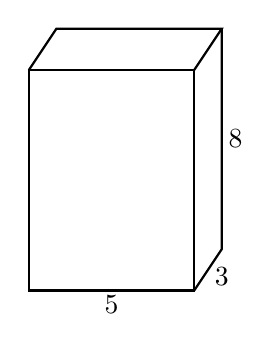
\begin{tikzpicture}[scale=0.7]
      \draw [-, thick] (0,0)--(3,0)--(3,4)--(0,4)--cycle;
      \draw [-, thick] (0,4)--(0.5,4.75)--(3.5,4.75)--(3,4);
      \draw [-, thick] (3,0)--(3.5,0.75)--(3.5,4.75);
      \node at (3.75, 2.75){$8$};
      \node at (1.5, -0.25){$5$};
      \node at (3.5, 0.25){$3$};
    \end{tikzpicture}
  \end{columns} \vspace{0.5cm}
  \end{frame}

\section{4.3 Solve for a side \hfill 3 November \,}
  \begin{frame}{Learning Target: I can solve for a missing parameter}
    {HSG.CO.C.9 Prove theorems about lines and angles  \hfill \alert{4.3 Thursday 3 November}}
    \begin{block}{Do Now}
      \begin{enumerate}
        \item Find the area of a circle with radius $r=10$, in terms of $\pi$
        \item Find the radius of a circle with area $A=49 \pi$
      \end{enumerate}
    \end{block}
      Lesson: Using algebra to solve problems, Deltamath practice \\
      Homework: Handout practice with volume calculations
  \end{frame}

\begin{frame}{Muhammad ibn Musa al-Khwarizmi - the ``father'' of algebra}
  {Persian 780 - 847 AD worked in Baghdad during the ``Islamic golden age''}
  \begin{description}
    \item[Algebra] Mathematics with symbols (named after al-Khwarizmi's book, al-jabra)
    \item[Algorithm] Logical steps to solve a problem (comes from his name)
    \item[Unknown] A symbol or letter representing a number, $x$, $y$, $a$, $\pi$, $\theta$
    \item[``reduction''] Cancellation of like terms on opposite sides of the equation
  \end{description}
    \center
    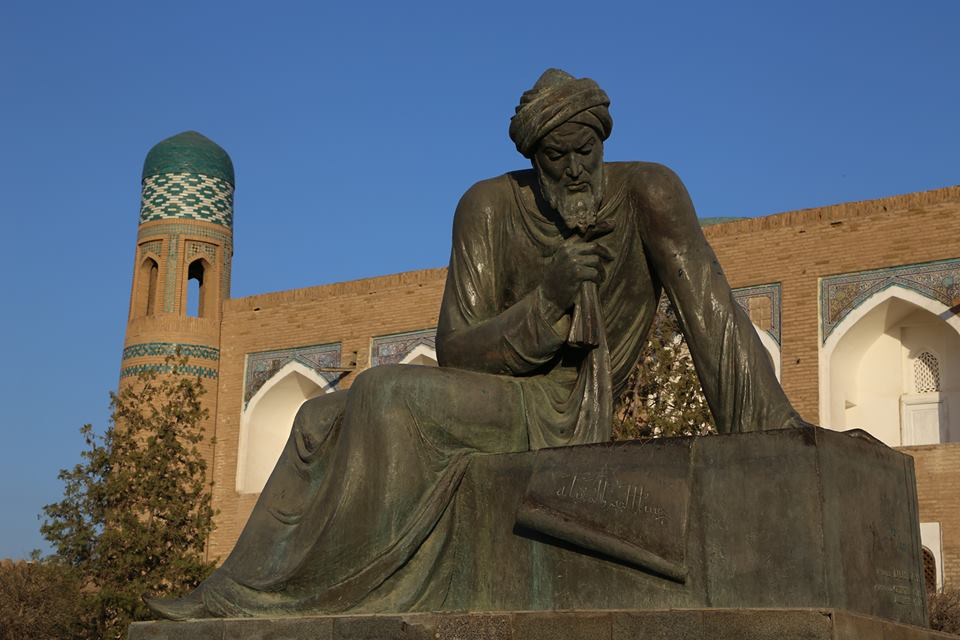
\includegraphics[width=0.6\textwidth]{../graphics/al-Khwarizmi_960-640.jpg}
\end{frame}

\begin{frame}{``Solve for $x$'' or ``isolate the variable''}
  {The algorithm developed by al-Khwarizmi}
  \begin{description}
    \item[Operation] Combine two numbers (multiplication or addition, for example)
    \item[Identity] 0 for addition, 1 for multiplication. 
      $$a+0=a \text{ and } a \times 1 = a$$
    \item[Inverse] Two values that make the identity for an operation. 
      $$a + (-a)=0 \text{ and } a \times \frac{1}{a}=1$$
  \end{description}
  $$a = b \Longleftrightarrow a+c = b+c$$
\end{frame}

\begin{frame}{Multiplying and dividing fractions}
  \begin{description}
    \item[Rational numbers] those that can be expressed as fractions, $\displaystyle \frac{p}{q} \in \mathbb{Q}$
    \item[Numerator] The top number in a fraction, \emph{dividend}, $p$
    \item[Denominator] \emph{Divisor}, bottom number in a fraction, $q$
    \item[Reciprocal] The multiplicative inverse
    \item[Division] Means to multiply by the reciprocal. $a \div b = \frac{a}{b} = a \times \frac{1}{b}$
  \end{description}
  To multiply fractions, multiply the numerators and denominators
  $$\frac{a}{b} \times \frac{c}{d} =\frac{a \times c}{b\times d}  $$
  To divide fractions, multiply by the reciprocal
  $$\frac{a}{b} \div \frac{c}{d} = \frac{a}{b} \times \frac{d}{c} = \frac{a \times d}{b\times c}  $$
  \end{frame}

\section{4.4 Surface area \hfill 4 November \,}
  \begin{frame}{Learning Target: I can calculate the surface area of a rectangular prism}
    {HSG.CO.C.9 Prove theorems about lines and angles  \hfill \alert{4.4 Friday 4 November}}
    \begin{block}{Do Now: Lumber used in construction called a ``two-by-four'' is actually \\
      $3 \frac{1}{2}$ inches by $1 \frac{1}{2}$ inches by 8 feet long.}
      \begin{enumerate}
        \item Find the area of the rectangular cross section, $3 \frac{1}{2}$ inches by $1 \frac{1}{2}$ inches
        \item Find the area of a triangular wedge cut from a two-by-four that is $3 \frac{1}{2}$ inches by one foot long.
      \end{enumerate}
    \end{block}
      Lesson: Surface area definition, formula; adding fractions \\
      Homework: Deltamath practice \\
      Extension: Deltamath absolute value, percent error
  \end{frame}

\begin{frame}{\emph{Surface area} is the combined total area of the faces of a polyhedron}
  \begin{columns}
    \column{0.7\textwidth}
    \begin{description}
      \item[Surface area] The total area of the outside of a solid
    \end{description}
    Given a rectangular prism with dimensions $l$, $w$, and $h$ the surface area is the sum of the six faces:
      $$S.A. = 2lw + 2lh + 2wh$$
      $$ = 2(5 \times 3) + 2(5 \times 8) + 2(3 \times 8)$$
      $$ = 158 \text{ square units} $$
    \column{0.3\textwidth}
    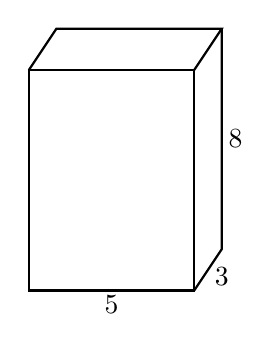
\begin{tikzpicture}[scale=0.7]
      \draw [-, thick] (0,0)--(3,0)--(3,4)--(0,4)--cycle;
      \draw [-, thick] (0,4)--(0.5,4.75)--(3.5,4.75)--(3,4);
      \draw [-, thick] (3,0)--(3.5,0.75)--(3.5,4.75);
      \node at (3.75, 2.75){$8$};
      \node at (1.5, -0.25){$5$};
      \node at (3.5, 0.25){$3$};
    \end{tikzpicture}
  \end{columns} \vspace{0.5cm}
\end{frame}

\begin{frame}{Adding and subtracting fractions}
  To add fractions with the same denominator, add the numerators.
  $$\frac{a}{c} + \frac{b}{c} =\frac{a + b}{c}$$
  \begin{description}
    \item[Equivalent fractions] Fractions that are equal. 
    $$\frac{a}{b} = \frac{a}{b} \times \frac{c}{c} = \frac{ac}{bc}$$
    \item[LCM] Lowest Common Multiple, for two fractions, multiples of the denominators that are equal.
    \item[Mixed fraction] A whole number and a fraction. e.g. $3 \frac{1}{2}$
  \end{description}
  \end{frame}

\begin{frame}{Adding fractions with different denominators}
  First convert to equivalent fractions with a common denominator. e.g. find
  $$\frac{1}{3} + \frac{1}{2}$$
  Convert to sixths
  $$\frac{1}{3} \times \frac{2}{2} = \frac{2}{6} \text{ and } \frac{1}{2} \times \frac{3}{3} = \frac{3}{6}$$
  Add these equivalent fractions instead:
  $$\frac{2}{6} + \frac{3}{6} = \frac{5}{6} $$
  \end{frame}

\section{4.5 Spheres, cones, pyramids \hfill 10 November \,}
\begin{frame}{Learning Target: I can calculate the volume of spheres, cones, and pyramids}
  {HSG.CO.C.9 Prove theorems about lines and angles  \hfill \alert{4.5 Thursday 10 November}}
  Do Now: Find the volume of a $3 \frac{1}{2}$ inch long scrap of a ``two-by-four''. \\
    (remember, the actual cross section is $3 \frac{1}{2}$ inches by $1 \frac{1}{2}$ inches) \\[0.5cm]
    Lesson: More volume formulas; exponent review \\
    Homework: Deltamath practice \\
    Extension: Deltamath exponent rules
\end{frame}

\begin{frame}{Volume of a cone or pyramid is one-third of a prism} 
  Given a base with area $B$ and a height $h$, \\
  the volume of a cone or pyramid is $V= \frac{1}{3} B \times h$
  \vspace{0.5cm}
  \begin{columns}
    \column{0.6\textwidth}
    \begin{description}
      \item[Rectangular] $V= \frac{1}{3} (l \times w \times h)$
      \item[Square] $V= \frac{1}{3} (s^2 \times h)$
      \item[Cone] $V= \frac{1}{3} (\pi r^2 \times h)$ 
    \end{description}
    \column{0.4\textwidth}
    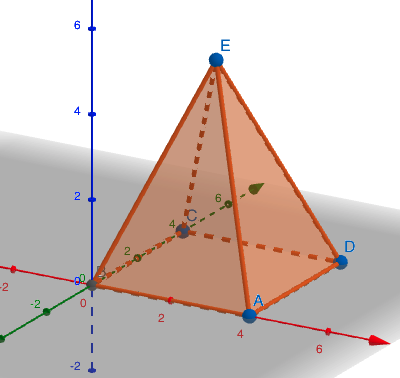
\includegraphics[width=0.8\textwidth]{../graphics/04pyramid.png}
  \end{columns} \vspace{0.5cm}
  \end{frame}

\begin{frame}{Volume and surface area of a sphere is a function of $\pi$} 
  Given a sphere with radius $r$
  \vspace{0.5cm}
  \begin{columns}
    \column{0.7\textwidth}
    \begin{description}
      \item[Sphere] A ball or globe shape
      \item[Volume] $V= \frac{4}{3} \pi r^3$
      \item[Surface area] $S.A.= 4 \pi r^2$ 
    \end{description}
    \column{0.3\textwidth}
    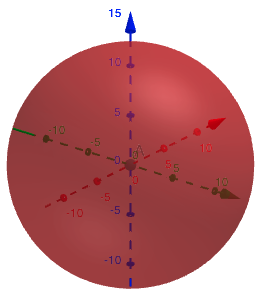
\includegraphics[width=0.8\textwidth]{../graphics/04sphere.png}
  \end{columns} \vspace{0.5cm}
  \end{frame}
  
\begin{frame}{Exponents mean repeated multiplication} 
  \vspace{0.5cm}
  \begin{description}
    \item[Superscript] ``Writing above,'' used for exponentiation. $x^2$
    \item[Subscript] ``Writing below,'' used for labeling or naming. $x_2$
  \end{description}
    Multiplying exponents with the same base
    $\underbrace{\overbrace{a \times a \times a}^3
    \times \overbrace{a \times a}^2}
    _\text{5} = x^6$

  \end{frame}

\end{document}